\documentclass{beamer}
% Include the preamble
\usepackage{graphicx}
\usepackage{hyperref}
\usepackage{listings}
\usepackage{xcolor}
\usepackage[utf8]{inputenc}

\usepackage[T1]{fontenc}
\usepackage[utf8]{inputenc}
\usepackage{textcomp}

\graphicspath{{../media/}}
\usepackage{tikz}
\usetikzlibrary{calc,patterns.meta}
% To provide total amount of sections throughout the document
\usepackage{totcount}
% Registers de total amount of sections (see https://tex.stackexchange.com/a/192506/141947)
\regtotcounter{section}
% To be able to refer to sections when needed
\usepackage{nameref}



% Redefinition of the \section command so that each one is labeled \label{sec:n} where n is its index 
\let\oldsection\section
\renewcommand{\section}[2][\relax]{%
    \ifx#1\relax
      \oldsection{#2}%
    \else
      \oldsection[#1]{#2}%
    \fi%
    \label{sec:\thesection}%
}

% ADDED:
\let\oldsubsection\subsection
\renewcommand{\subsection}[2][\relax]{%
    \ifx#1\relax
      \oldsubsection{#2}%
    \else
      \oldsubsection[#1]{#2}%
    \fi%
    \label{subsec:\thesection-\thesubsection}%
}

% Definition of custom colors based on the initial figure of the bar by the OP
\definecolor{myblue}{HTML}{57AED1}
\definecolor{mygreen}{HTML}{8BC53F}
\definecolor{mygray}{HTML}{DDDDDD}

% Definition of custom tikz styles in order to ease readability
\tikzset{
    % Bar style (Argument : color)
    sectionbar/.style={
        % Filling with one color as a preaction, in order to avoid reset by the pattern color
        preaction={fill=#1!70},
        % Application of the line pattern on to of the fill
        pattern={Lines[angle=45,distance={6pt},line width=3pt]},pattern color=#1
    },
    % Node style (Arguments : color, section number)
    sectionnode/.style 2 args={
        fill=#1,
        draw=white,
        thick,
        circle,
        text=white,
        radius=10pt,
        % Display of the section name below the cicle
        label={[text=#1,align=center]below:\nameref{sec:#2}\\~},% CHANGED
        },
    % ADDED: Node style (Arguments : color, section number, subsection number)
    sectionnodeWithSubsection/.style n args={3}{
        fill=#1,
        draw=white,
        thick,
        circle,
        text=white,
        radius=10pt,
        % Display of the section name and the subsection name below the cicle
        label={[text=#1,align=center]below:\nameref{sec:#2}\\-- \nameref{subsec:#2-#3} --},
        }
}


% Actual definition of the colorbar based on Gonzalo Medina's initial proposal
\makeatletter
    \def\pbar@progressbar{} % the progress bar
    \newcount\pbar@tmpcnta% auxiliary counter
    \newcount\pbar@tmpcntb% auxiliary counter
    \newdimen\pbar@pbht %progressbar height
    \newdimen\pbar@pbwd %progressbar width
    \newdimen\pbar@tmpdim % auxiliary dimension
    \pbar@pbwd=\linewidth
    \pbar@pbht=4pt

% The progress bar
\def\pbar@progressbar{%
    \pbar@tmpcnta=\value{section} % tmpcnta stores the section number
    \pbar@tmpcntb=\totvalue{section} % tmbcountb sotres the total amount of sections
    \advance\pbar@tmpcntb by 1 % tmbcountb is advanced by 1 in order to have the last bar segment after the last node

    \begin{tikzpicture}[very thin]
        % Clipping scope to avoid tests for the bar dimensions
        \begin{scope}
        % Clipping path
        \path[rounded corners=2pt,clip] (0pt,{-\pbar@pbht/2}) rectangle (\pbar@pbwd,{\pbar@pbht/2});
        % Gray bar (from 0 to last section)
        \path[sectionbar=mygray] (0pt,{-\pbar@pbht/2}) rectangle (\linewidth,{\pbar@pbht/2});
        % Blue bar (from 0 to the current section)
        \path[sectionbar=myblue] (0pt,{-\pbar@pbht/2}) rectangle ({(\pbar@tmpcnta-0.5)*\linewidth/\pbar@tmpcntb},{\pbar@pbht/2});
        % Green bar (from current to next section)
        \path[sectionbar=mygreen] ({(\pbar@tmpcnta-0.5)*\linewidth/\pbar@tmpcntb},{-\pbar@pbht/2}) rectangle ({(\pbar@tmpcnta+0.5)*\linewidth/\pbar@tmpcntb},{\pbar@pbht/2});
        \end{scope}
        % Drawing of the nodes on top of the bars, based on the number of the current section
        \foreach \secnumber in {1,...,\totvalue{section}}{
            % Number is lower, section is past, blue color
            \ifnum\secnumber<\pbar@tmpcnta
                \node[sectionnode={myblue}{\secnumber}] at ({(\secnumber-0.5)*\linewidth/\pbar@tmpcntb},0) {\strut\secnumber};
            \fi
            % Number is equal, section is current, green color
            \ifnum\secnumber=\pbar@tmpcnta
                % CHANGED:
                % if we have a current subsection, show current subsection
                \ifnum\thesubsection>0
                    \node[sectionnodeWithSubsection={mygreen}{\secnumber}{\thesubsection}] at ({(\secnumber-0.5)*\linewidth/\pbar@tmpcntb},0) {\strut\secnumber};
                \else
                    \node[sectionnode={mygreen}{\secnumber}] at ({(\secnumber-0.5)*\linewidth/\pbar@tmpcntb},0) {\strut\secnumber};
                \fi
            \fi
            % Number is larger, to be done section, gray color
            \ifnum\secnumber>\pbar@tmpcnta
            \node[sectionnode={mygray}{\secnumber}] at ({(\secnumber-0.5)*\linewidth/\pbar@tmpcntb},0) {\strut\secnumber};
            \fi
        }
  \end{tikzpicture}%
}

\addtobeamertemplate{headline}{}
{%
  \begin{beamercolorbox}[wd=\paperwidth,ht=13ex,center,dp=1ex]{white}% CHANGED: value of ht
    \pbar@progressbar%
  \end{beamercolorbox}%
}
\makeatother

\title{Docker: An Introduction}
\author{JC Cruz}
\date{\today}

\begin{document}

\frame{\titlepage}

\section{Problem Statement}

\begin{frame}{Problem Statement}
    \begin{itemize}
        \item You're on your local laptop with Windows or the latest Ubuntu image 24.04
        \item Your supervisor asks you to validate the results of some software from another group
        \item The group emails you their source code and scripts but it turns out it was developed on Ubuntu 14.04 (which released in 2014 and had EOL in April 2024) and does not work on your host PC
        \item What to do now?
    \end{itemize}
    
\includegraphics[width=0.8\textwidth]{angry_boss.png}
\end{frame}

\section{Solutions}

\begin{frame}{Solutions}
    \begin{enumerate}
        \item Setup and configure on some old HDD or SSD
        \begin{itemize}
            \item Takes time, hardware
            \item No guarantee of out-of-box compatibility
        \end{itemize}
        \item Boot into VMware with the correct OS
        \begin{itemize}
            \item No guarantee of out-of-box compatibility
            \item Can be pretty slow
        \end{itemize}
        \item Use Docker
        \begin{itemize}
            \item Quick setup
            \item Consistent environment across different machines
            \item Lightweight compared to VMs
        \end{itemize}
    \end{enumerate}
    
\includegraphics[width=0.8\textwidth]{docker_anime.png}
\end{frame}

\section{Docker Background}

\begin{frame}{Docker Background}
    \begin{itemize}
        \item Launched in 2013
        \item Open-source platform for containerization
        \item Allows applications to run in isolated environments called containers
        \item Uses host OS kernel, making it more efficient than VMs
    \end{itemize}
    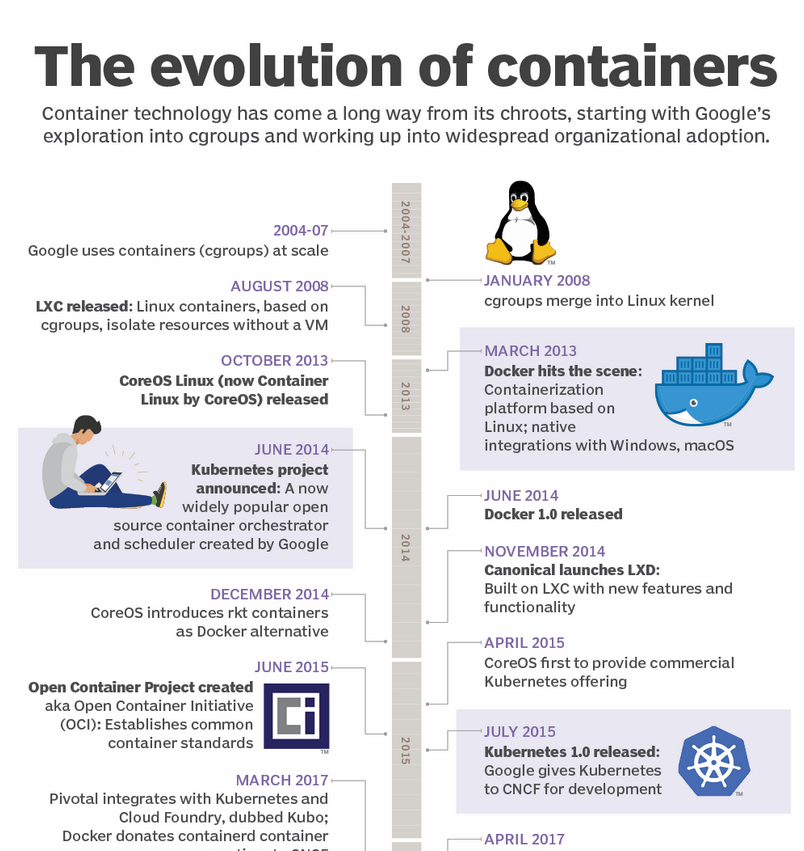
\includegraphics[width=0.8\textwidth]{timeline.png}
\end{frame}

\section{Benefits of Docker}

\begin{frame}{Benefits of Docker}
    \begin{itemize}
        \item Consistency across development, testing, and production environments
        \item Faster deployment and scaling
        \item Better resource utilization compared to VMs
        \item Simplified dependency management
        \item Easier application isolation and security
        \item Avoid problem of "it runs on my machine"
    \end{itemize}
    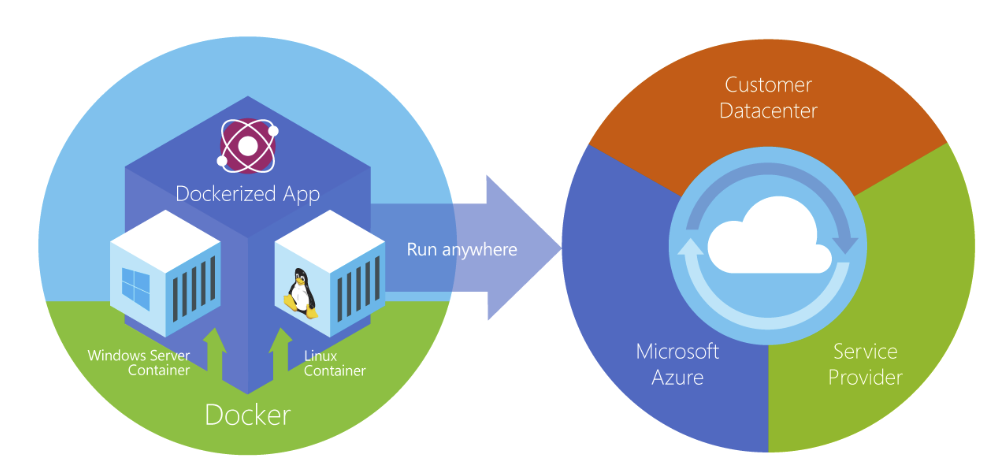
\includegraphics[width=0.8\textwidth]{diagram.png}
\end{frame}

\section{Docker Architecture}

\begin{frame}{Docker Architecture}
    \begin{itemize}
        \item Docker Engine: Core component that builds and runs containers
        \item Docker Client: CLI tool for interacting with Docker
        \item Docker Daemon: Background service managing Docker objects
        \item Docker Registry: Storage for Docker images (e.g., Docker Hub)
        \item Docker Objects: Images, containers, networks, volumes
    \end{itemize}
    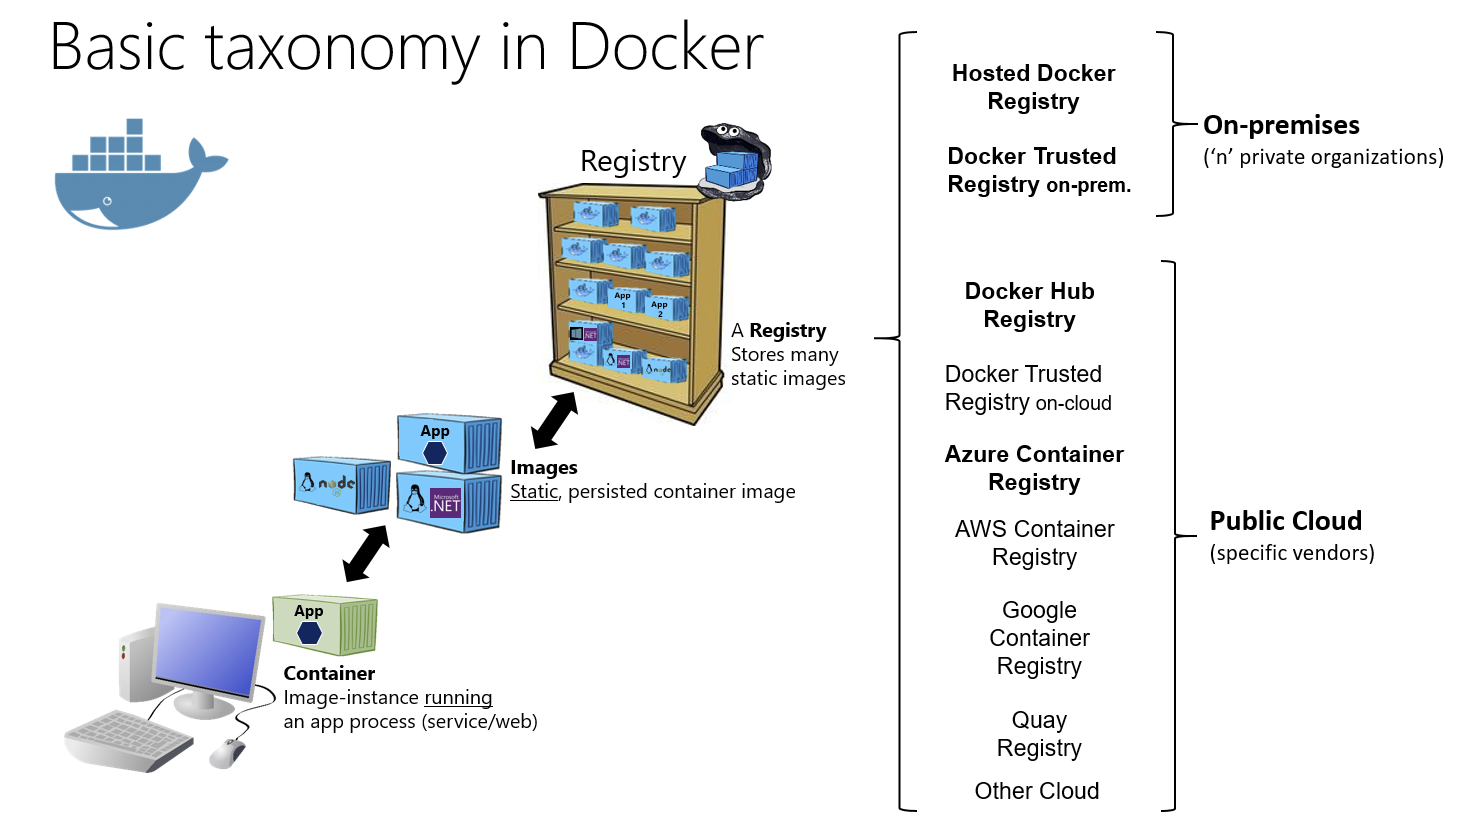
\includegraphics[width=0.8\textwidth]{taxonomy.png}
\end{frame}

\section{Important File Types}

\begin{frame}{Important File Types}
    \begin{itemize}
        \item Dockerfile (Dockerfile)
        \begin{itemize}
            \item Defines a single container
            \item Used to build custom images
        \end{itemize}
        \item Docker Compose (docker-compose.yaml)
        \begin{itemize}
            \item Orchestrates multiple containers
            \item Manages application-wide settings and networking
        \end{itemize}
        \item Docker ignore (.dockerignore)
        \begin{itemize}
            \item Specifies files to be excluded from the build context
        \end{itemize}
    \end{itemize}
    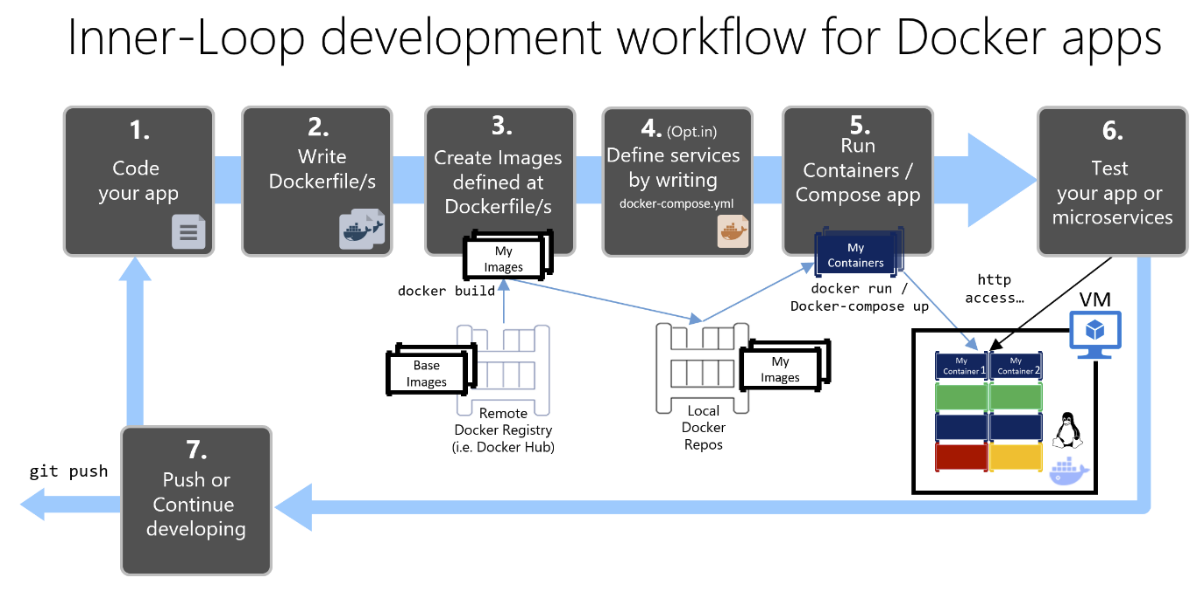
\includegraphics[width=0.8\textwidth]{workflow.png}
\end{frame}

\section{Docker Commands}

\begin{frame}{Docker Commands}
    \begin{itemize}
        \item \texttt{docker build}: Build an image from a Dockerfile
        \item \texttt{docker run}: Create and start a container from an image
        \item \texttt{docker pull}: Download an image from a registry
        \item \texttt{docker push}: Upload an image to a registry
        \item \texttt{docker ps}: List running containers
        \item \texttt{docker images}: List available images
        \item \texttt{docker stop}: Stop a running container
        \item \texttt{docker rm}: Remove a container
        \item \texttt{docker rmi}: Remove an image
    \end{itemize}
\end{frame}

\section{Docker Compose Commands}

\begin{frame}{Docker Compose Commands}
    \begin{itemize}
        \item \texttt{docker-compose up}: Create and start containers
        \item \texttt{docker-compose down}: Stop and remove containers, networks, images, and volumes
        \item \texttt{docker-compose build}: Build or rebuild services
        \item \texttt{docker-compose ps}: List containers
        \item \texttt{docker-compose logs}: View output from containers
        \item \texttt{docker-compose exec}: Run commands in a running container
    \end{itemize}
\end{frame}

\section{Example: Python Development}

\begin{frame}[fragile]{Example: Python Development}
    \begin{itemize}
        \item Directory structure:
    \end{itemize}
    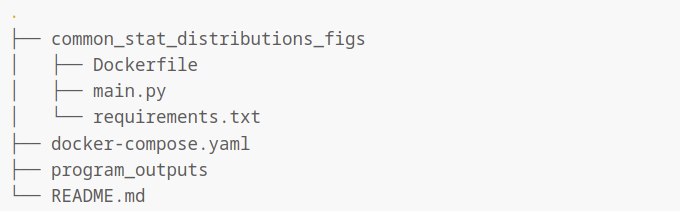
\includegraphics[width=0.8\textwidth]{py_dir_struct.png}
\end{frame}

\begin{frame}[fragile]{Dockerfile}
    \begin{verbatim}
# Use an official Python runtime as a parent image
FROM python:3.8.19-bookworm

# Avoid prompts from apt
ENV DEBIAN_FRONTEND=noninteractive

# Set the working directory in the container
WORKDIR /container_workspace

# Install system dependencies
RUN apt-get update && apt-get install -y \
    gcc \
    && rm -rf /var/lib/apt/lists/*

# Copy the current directory contents into the container
COPY . /container_workspace/

# Install any needed packages specified in requirements.txt
COPY requirements.txt /container_workspace/
RUN pip install --no-cache-dir -r requirements.txt

# Run main.py when the container launches
CMD ["python", "main.py"]
    \end{verbatim}
\end{frame}

\begin{frame}[fragile]{docker-compose.yaml}
    \begin{verbatim}
version: '3'
services:
  python_plotting_script:
    build: ./common_stat_distributions_figs
    volumes:
      - ./program_outputs:/container_workspace/program_outputs
    \end{verbatim}
\end{frame}

\begin{frame}{Building and Running}
    \begin{itemize}
        \item Building:
        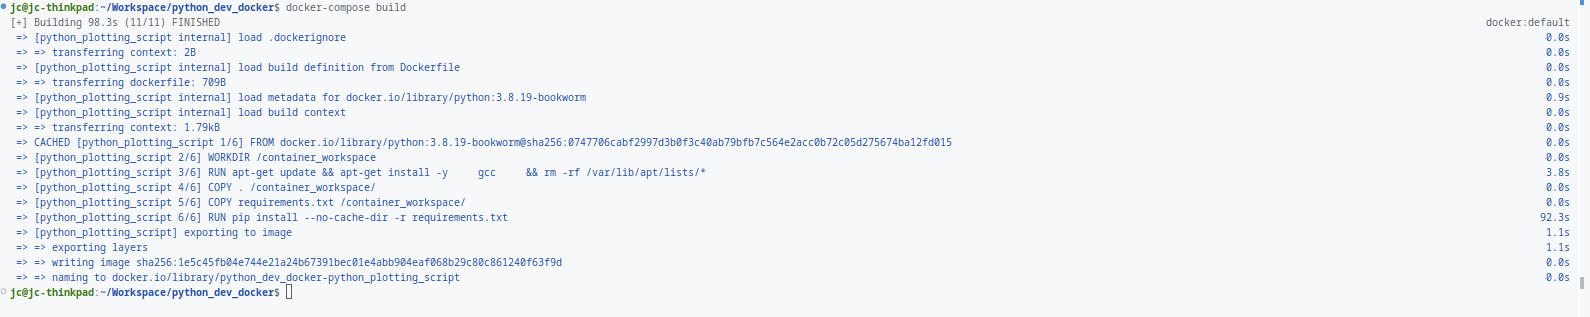
\includegraphics[width=0.8\textwidth]{py_build.png} 
        \item Running:
        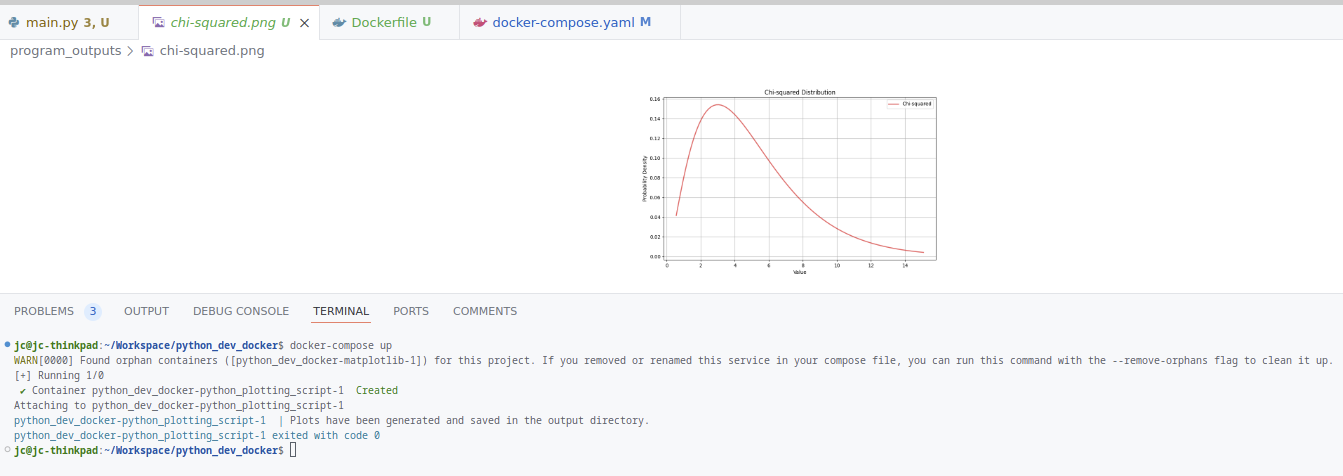
\includegraphics[width=0.8\textwidth]{py_run.png}
        \item What if I try to run locally?
        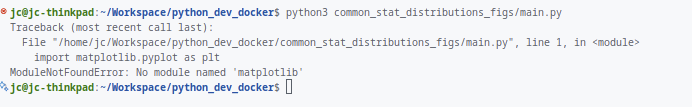
\includegraphics[width=0.8\textwidth]{py_fail.png}
    \end{itemize}
\end{frame}

\end{document}